%pygmentize_options: -O startinline=True

\chapter{Analysing PHP Code}

    The PHP programming language first appeared in 1995\cite{phphist}. Over the years 
    the language has evolved and so have the ways programmers use it. 
    This project focuses on PHP version 5.5\footnote{From this point, 
    if the PHP version is not stated explicitly, it is implicitly 5.5.} 
    and the aim for the analysis 
    is to work well on PHP source code written in an object oriented style, 
    using modern PHP patterns and idioms that are described later in 
    this text. The analysis, however, should provide correct results for 
    any valid PHP code of any PHP version. We do not focus only on websites, but also on 
    PHP libraries and frameworks that by themselves do not contain 
    any PHP files that produce HTML or any other output for the user.
    
    The following section PHP Semantics describes some important parts 
    of the semantics of the PHP programming language, especially those 
    that represent a challenge for static analysis.

    Section Static Code Analysis gives a brief overview of existing 
    static analysis methods, especially Data Flow Analysis 
    (DFA)\cite{aho1985compilers}\cite{nielson1999principles}, 
    which has become a de-facto standard type of analysis for most of 
    the optimizing compilers and other more complex static analysis methods 
    are either directly based on DFA or on the ideas behind DFA. 
    This section includes references to relevant literature and 
    is not meant as a comprehensive description, but should provide a 
    context for the following section Control Flow for Phalanger Approach, 
    where we discuss how we used the existing techniques for the purposes 
    of our PHP code analysis.
    
    \section{PHP Semantics}

    \subsection{Dynamic Typing}
    In PHP, local or global variables, object fields and function or 
    method parameters are dynamically typed, which means that they 
    can hold values of completely different types at different 
    times of the execution.
    
    \subsection{Local Variables}
    Local variables in PHP do not need to be declared explicitly. 
    Instead the first usage of a variable is also its declaration. 
    If a variable's value is used before the variable got any 
    value assigned, then the interpreter generates a notice, 
    however the execution continues and value \code{null} is 
    used instead. A variable can get a value assigned to it when it 
    appears on a left hand side of an assignment or when a 
    reference to that variable is created, in which case it gets value 
    \code{null}, but no notice is generated. References are 
    discussed in one of the following subsections.

    The scope of a local variable is always its parent function not the 
    parent code block as in other languages like C or Java. 
    So in the following 
    example, the usage of variable \code{\$y} at the end 
    of the function can generate uninitialized variable notice, 
    however, if \code{\$x} was equal to \code{3}, 
    \code{\$y} will have a value although it 
    was declared in the nested code block.

%pygmentize_begin php
% function foo($x) {
%   if ($x == 3) { $y = 2; }
%   echo $y; // uninitialized variable if x != 3
% }
%pygmentize_end
    
    \subsection{Global and Local Scope}
    PHP distinguishes two scopes for variables: global scope and 
    local scope. Local scope is a scope of local variables 
    within a user defined routine.         
    Variables that are declared 
    in global scope, that is outside of a user defined routine, 
    are available anywhere in global scope and are called 
    global variables. Global variables are also available 
    in user defined routines as long as they are imported 
    into the routine's scope using the keyword \code{global}.
    
%pygmentize_begin php
% $g1 = 1;  // global variables g1 and g2
% $g2 = 2;
% function foo() {
%   global $g1;
%   echo $g1;   // prints the value of global variable g1
%   $g2 = 4;   // sets the value of local variable g2,
%   // because global variable g2 was not imported, 
%   // its value does not change
% }
%pygmentize_end

    Global variables can be imported and used in any user defined 
    routine. This means that even if we know some type information 
    about a global variable's value at some point in the analysed 
    code (e.g. straight after assignment to that variable), 
    any time another user defined routine is invoked, we 
    have to take into account that the other routine can 
    change the value of the global variable even if we do not 
    pass the global variable to the invoked routine 
    as an argument passed by reference.

    \subsection{Closures}
    PHP also supports anonymous functions. An anonymous function has its 
    own scope as any other function and its local variables are not visible 
    to the scope where it was declared. Variables from the parent 
    scope are available in the closure scope only if they are 
    explicitly imported to its scope and they can be captured 
    by value or by reference. Only the later represents a 
    challenge for the analysis, because any code that can 
    access the closure can invoke it and thus change the 
    values of variables imported to the closure's scope 
    by reference. By invoking a closure, we can influence 
    the values of variables in a completely different 
    and otherwise inaccessible scope.
    
    \subsection{References}
    References in PHP are similar, but not same, as pointers 
    in the C programming language. PHP has a special 
    operator \code{=\&} (assign by reference) that turns 
    the variable on the 
    left hand side into a reference to the 
    variable on right hand side. For example \code{\$a=\&\$b}, 
    after this, any assignment 
    to \code{\$a} will in fact change the 
    value of \code{\$b} and wherever 
    the value of \code{\$a} is used (e.g. in an expression), 
    the value of \code{\$b} is used instead.
    
    The variable the reference is pointing to is determined 
    in a transitive fashion, which means that if we assign 
    by reference another reference, the new reference will 
    point to where the other reference was pointing to, 
    but the intermediate link is lost. The following example 
    illustrates this.
    
%pygmentize_begin php
% $a =& $b;       // a points to b
% $c =& $a;       // c points to where a points, that is b
% $a =& $d;       // a points to d, but c still points to b
%pygmentize_end    

    \subsection{Arrays}
    Arrays in PHP do not have to be homogenous and 
    they can be indexed by either integers or strings.
    In fact, PHP arrays are hash maps rather than arrays 
    in the usual sense and that is also how they are 
    implemented internally. 
    
    String indexed heterogenous arrays are often used 
    as flexible ad-hoc structured data type. 
    Instead of defining a class 
    with required fields, one can use what would be a 
    field name as an index into an array. Such arrays 
    are usually indexed only with finite number of 
    constant string values. 
    
    In this light, it is no 
    surprise that using the subscribe operator 
    \code{[]} with string index on an object instance will 
    access the field with the same name as the index value.

    \subsection{Interesting Control Flow Structures}
    The \code{break} and \code{continue} statements with 
    optional numeric argument are supported in PHP in a 
    similar way as in other imperative programming 
    languages. There are, however, important differences 
    to be noted.
    
    Firstly, The numeric argument can be an arbitrary 
    expression in some of the older versions of PHP, in which 
    case we cannot statically determine the target of 
    the jump for the control flow resolution.
    
    Secondly, the \code{switch} statement is considered 
    a loop for the purposes of both \code{break} and 
    \code{continue}. The semantics of \code{break} 
    is intuitive. One of the meaningful use cases is to 
    break a loop from within a \code{switch} by 
    using \code{break 2}. The semantics of 
    \code{continue} statement 
    is perhaps not so intuitive: within a \code{switch} 
    it works the same way as \code{break}.
    
    \subsubsection*{Switch Statement Semantics} 
    The basic semantics of the \code{switch} statement in PHP is 
    again very similar to that of other standard imperative 
    programming languages. The \code{switch} statement in PHP 
    permits an arbitrary expression as the value to be used 
    for comparison with values of its \code{case} labels. Furthermore, 
    the values of \code{case} labels can also be arbitrary 
    expressions and because we are in a context of dynamic 
    programming language, they can again evaluate to a value 
    of any type at runtime.
    
    The switch expression is evaluated only once 
    at the beginning, and if it has an undefined value (undefined variable, 
    void function call), then the control flow goes directly 
    to the default item, without evaluating the expressions 
    in the case items. If the value is defined, then it is 
    one-by-one compared to the values that the 
    \code{case} labels evaluate to. If a \code{case} label evaluates 
    to \code{boolean} value, then it is used to decide whether to 
    jump to that \code{case} item or continue with evaluating 
    the value of the next \code{case} label. Note that the value of 
    switch expression is not compared to the \code{case} label value. 
    If a \code{case} label evaluates to a complex type (\code{object} or \code{array}), 
    it is ignored and evaluation continues with the next \code{case} label. 
    And finally, if a \code{case} label evaluates to an 
    \code{integer}, \code{float} or \code{string} value, it is 
    compared to the switch expression. All these expressions can 
    have side effects due to usage of assignments as expressions 
    or calls of functions with side effects. 
    
    PHP also permits placing the \code{default} label anywhere in between 
    the other \code{case} labels. This can be used for fall-back 
    to or from a \code{case} item as in the following code sample 
    that is abbreviated version of actual code taken from the 
    WordPress\cite{wordpress} code base.
    
%pygmentize_begin php
%switch ( $status ) {
%    default:
%    case 'install':
%        $actions[] = '<a class="install-now" ...';
%        break;
%    case 'update_available':
%        $actions[] = '<a class="install-now" ...';
%        break;
%    case 'newer_installed':
%    case 'latest_installed':
%        $actions[] = '<span class="install-now" ...';
%        break;
%}
%pygmentize_end    
    
    
    \subsection{Conditional Declarations}
    User defined functions, classes, etc. are declared in 
    a global scope in PHP, that is a scope where one can 
    as well place any arbitrary code. Therefore a declaration 
    can be wrapped in any control structure. 
    It is not allowed to redeclare once declared symbol, however.
    
    A typical use case is to dynamically import a file 
    that may provide some functions and then check, 
    using \code{function\_exists}, whether the functions were 
    indeed declared and if not, provide default implementation.
    This is a pre-object-oriented way of doing overriding and 
    is usually not to be found in modern projects. Nonetheless, 
    WordPress still relies on this pattern in parts of its code base.
    
    Although the mentioned pattern could be deemed as 
    reasonable and useful. This feature permits very problematic 
    code as in the following example that may or may not 
    crash on fatal errors ``Cannot redeclare foo()'' or 
    ``Call to undefined function foo()'' depending upon 
    the user input.
    
%pygmentize_begin php
%while ($_POST['a'] != 3) {
%   function foo() { return 5; }
%   $_POST['a'] = $_POST['b'];
%}
%echo foo();
%pygmentize_end        
    
                
    \subsection{Auto-loading}
    Historically, in PHP, in order to reference any symbol 
    from a different file, one had to import that 
    file explicitly. Newer versions of PHP support  
    customized auto-loading. A user defined routine 
    can be invoked by the runtime every time an 
    undefined class is referenced. 
    The auto-loading routine is then responsible for 
    importing the file(s) that contain the code of the 
    required class. 
    
    Auto-loading routine can use arbitrary logic to 
    determine what file(s) to import, in fact, it can 
    execute arbitrary code. Typical 
    pattern used for example in 
    Zend Framework\cite{zendframework} before namespaces were 
    introduced to PHP is to have a file per class and use 
    class names in form of 
    \code{CodeFolder1\_SubFolderName\_FileName} for 
    a class placed in file 
    \filepath{CodeFolder1\SubFolderName\FileName.php}.
    
    \subsection{PHPDoc Annotations}
    Although not part of the official PHP syntax, 
    there is a widely recognized format for documentation 
    comments of JavaDoc style called PHPDoc. PHPDoc comments 
    may contain type information that cannot be expressed using 
    PHP syntax. For example, PHP allows ``type hints'' 
    for routine parameters, but only for class types, 
    not for primitive types like \code{int}. However, 
    primitive type expectations can be included in the 
    documentation comments. The important difference 
    is that PHP will throw an exception at runtime if 
    a routine is invoked with a parameter of different 
    type than what its ``type hint'' is. The documentation
    comments, on the other hand, are of course ignored 
    by the runtime.
    
    The PHPDoc defines a fairly advanced syntax for expressing 
    type information. It supports multiple 
    primitive and class types, homogenous and heterogenous arrays as well 
    multidimensional arrays, and some constants like \code{false}.
    For example, in the following code the documentation 
    comment tells us that function \code{foo} can return 
    either \code{null}, or \code{false} (but should never 
    return \code{true}), or an array of \code{integer} values.
    
%pygmentize_begin php
% /**
%  * @return null|false|int[]
%  */
% function foo() { ...
%pygmentize_end
    
    \section{Static Code Analysis}       
        Static analysis of source code is an analysis that is performed without 
        executing the code. This means that we do not need to have a
        web server, for example, in order to analyse code of a web application. 
        We can also guarantee some properties of the analysis that would not 
        be possible to guarantee if we executed the code. Namely the halting property and 
        upper bounds on time and space complexity. Arbitrary code may not 
        halt if executed, but static analysis of such code can still halt 
        and give results.
        
        Static analysis can be used to get possible types of an expression in 
        a dynamically typed language, to find out expressions that have constant 
        value through constant propagation and many other problems. 
        Static analyses usually do not give accurate solution, it is an approximation, 
        which can be an over-approximation or an under-approximation and it is up 
        to the designer and user of the analysis which one is acceptable for 
        his or her\footnote{``His'' or ``he'' 
        should be read as ``his or her'' or ``he or she'' through the rest of the text.} 
        purposes.
        
        %---------------------------------------------------------------------------------------
        \subsection{Program State}
        Execution of a program can be seen as a series of transformations of 
        the program state. Each individual program instruction, when executed, 
        can change the program state and produces its \emph{output state}.         
        How exactly is defined by the instruction's semantics and it typically 
        depends on the \emph{input state}, which is a program state produced 
        by the previously executed instruction. 
        
        The goal of a static analysis is to devise some useful piece of information 
        about how instruction $i$ can change the program state, so that it can 
        be used for program optimization or to reveal potentially problematic 
        instructions. For example, if assignment $a=4/b$ always assigns 
        constant value $1$ to $a$, because $b$ happens to be equal to $4$ 
        in any possible program state preceding $a=4/b$, we can change 
        $a=4/b$ to $a=1$, which has the same affect to the program state. 
        If we instead found out that $b$ is always equal to $0$, we would 
        know that this instruction will cause an exception.
        
        The result we expect from a static analysis is, for each instruction 
        in the program, provide some useful property of program state transformation 
        that always holds every time the instruction is executed. 
        The analyses differ in the properties they compute. 
        We will call such computed property a \emph{data-flow}.
        
        
        %---------------------------------------------------------------------------------------
        \subsection{Control Flow Graph.} 
        DFA is typically performed on a control flow graph, 
        although there exist approaches to DFA 
        without explicit control flow graph 
        construction \cite{mohnen2002graph}.
        
        Control flow graph nodes, also called basic blocks, 
        are program statements that are always executed sequentially. 
        Directed edges represent the control flow between basic blocks, 
        for example, jumps in the control flow due to conditionals, 
        \code{goto} statements or any other statements that can change 
        the flow of the program.        
        Control flow graphs usually contain two special nodes: 
        entry node and exit node. The entry node does not have any 
        incoming edges and all the paths lead to the exit node.        
        An example of a control flow graph is given in figure \ref{cfg}.
        
\begin{table}[h]
  \begin{tabular}{ l | m{6cm} }
  \centering
    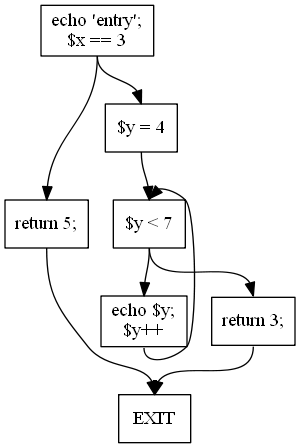
\includegraphics[scale=0.7]{img/cfg.png}
  &
 
\begin{minipage}{6cm}
%pygmentize_begin php
%   echo 'entry';
%   if ($x == 3)
%       $y = 4;
%   else
%       return 5;
%        
%   while ($y < 7) {
%       echo $y;
%       $y++;
%   }
%
%   return 3;
%pygmentize_end
\end{minipage}

  \\
  \end{tabular}
  \caption{Control flow graph\label{cfg}}  
\end{table}        
        
        %---------------------------------------------------------------------------------------
        \subsection{Transfer functions}
        
        We say that the input state of a statement is associated with 
        the \emph{program point before} the statement and the output state 
        is associated with the \emph{program point after} the statement. 
        Our aim is to calculate \emph{data-flow} value for both 
        program points for each statement, denoted $IN(s)$ and $OUT(s)$ for 
        a statement $s$.
        
        \subsubsection*{Single Statement}
        
        We can express the \emph{data-flow} for \emph{program point after} 
        a statement as a function of the \emph{data-flow} of 
        \emph{program point before} the statement, also called \emph{transfer function}. 
        Formally if $f_t$ is a \emph{transfer function}, then $f_t(IN(s))=OUT(s)$.
        Each type of statement will have a different \emph{transfer function} 
        that will reflect the semantics of the statement. 
        
        Example: our analysis tracks type of local variables, so the \emph{data-flow} 
        is a map from variable names to their type. In such setting, a \emph{transfer function} 
        for assignment statement \code{\$a=\$b}, will take the input \emph{data-flow} 
        $flow_{in}$ and will return $flow_{out}$, such that $flow_{out}(x)=flow_{in}(x)$ for 
        every variable name $x$, except for $flow_{out}(\$a)=flow_{in}(\$b)$. In other words, 
        the type of all the variables stays the same, except for \code{\$a} whose type 
        changes to whatever is the type of \code{\$b} is. 
        
        In practice, there is only one \emph{transfer function} for all the assignment 
        statements that is parametrized by the left-hand side and right-hand side of 
        the assignment. And in general, each statement in the programming language has 
        usually its ``meta'' \emph{transfer function} that is parametrized not only 
        by the input \emph{data-flow}, but by the statement structure.
        
        \emph{Transfer functions} are often described in the form of inference rules. 
        An example of an inference rule can be 
        ``if the type of variable \code{b} is \code{Integer} in state $S_1$, 
        then after executing statement \code{a=b}, we get a new state $S_2$ that 
        is the same as $S_2$ except variable \code{a} is of type \code{Integer} in $S_2$''. 
        Those rules can be more formally described with the following notation        
        $$
        \infer{[a=b, S_1] \rightarrow S_2, S_2 \vdash a : Integer}{S_1 \vdash b : Integer}
        $$        
        where above the horizontal line we have hypothesis and below is 
        the conclusion. The exact notation is not important, we will be using it 
        intuitively to illustrate the ideas that we describe.
        
        %[a=b,s1] => s2,a:Integer || b:integer \in S2
        
        \subsubsection*{Statement Interaction}
        
        The \emph{data-flow} for \emph{program point before} a statement 
        depends on the \emph{data-flow} of \emph{program point after} the 
        last executed statement. Let us consider a basic block $B$ with 
        statements $s_0, s_1, ..., s_n$.
        
        In the case of any $s_i \neq s_0$, that is any statement but 
        the first one, there is only one statement whose execution 
        can precede the execution of $s_i$ and that is the previous statement 
        in the sequence: $s_{i-1}$. So we have $IN(s_i) = OUT(s_{i-1})$ 
        for $i\in{[1..n]}$. 
        
        In fact, thanks to this property, we can define \emph{transfer function} 
        $f_B$ of a basic block as composition of transfer functions of 
        its statements. Formally: 
        
        \[ f_B = f_{s_n} \circ f_{s_{(n-1)}} \circ ... f_{s_0} \]
        
        where $f_{s_i}$ is the transfer function for statement $s_i$.            
        Furthermore, we denote \emph{data-flow values} of basic block as 
        $IN(B)=IN(s_1)$ and $OUT(B)=OUT(s_n)$. From the definitions we can 
        observe simple identities: 
        
        \[ f_B(IN(s_1))=f_B(IN(B))=OUT(B)=OUT(s_n) \]
        
        The first statement $s_1$ of the basic block has to be 
        handled differently. Its execution can be preceded by 
        execution of the last statement of any of 
        the basic blocks $B_1, B_2, ..., B_m$ that precede basic block 
        $B$ in the control flow graph. One of the possibilities to deal with 
        this, is to combine \emph{data-flows} $OUT(B_1), ..., OUT(B_m)$ into 
        single \emph{data-flow} that approximates all of them. 
        Nonetheless, the way the \emph{data-flows} are combined depends 
        on the concrete \emph{data-flow} type and thus 
        should be defined by the analysis. We denote the function to 
        combine \emph{data-flows} as $\mathit{MEET}$. 
        
        \subsubsection*{Equations for Data-Flow}
        
        When we put everything together, we get a set of equations:
        \begin{align*}
            OUT(B_i) &= f_{B_i}(IN(B_i)) \\
            IN(B_i) &= \mathit{MEET}(OUT(P_0), ..., OUT(P_m)) \\ 
        \end{align*}
        where $P_0, ..., P_m$ are predecessors of $B_i$ in the 
        control flow graph. The analysis must also define value 
        of $IN(START)$, that is \emph{input state} for the 
        initial node, which does not have any predecessors.
        
        \subsubsection*{Example}
        We will illustrate the system of \emph{data-flow} equations on a 
        simple example. The subject of our analysis will be the 
        type of the variable \code{\$i} in the code sample in figure \ref{dfacfg}.
        
        \emph{Data-flow} will be a set of possible types of variable $i$ and 
        initial \emph{data-flow} of the start node will be an empty set.

\begin{table}[h]
  \begin{tabular}{ l | m{6cm} }
  \centering
    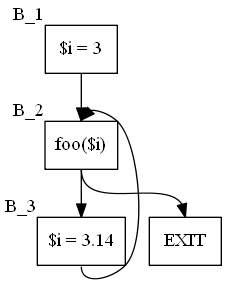
\includegraphics[scale=0.7]{img/dfa-cfg.png}
  &
 
\begin{minipage}{6cm}
%pygmentize_begin php
%   $i = 3;
%   while (foo($i)) {
%       $i = 3.14;
%   }
%   // exit
%pygmentize_end
\end{minipage}

  \\
  \end{tabular}
  \caption{Code for Data-Flow Example\label{dfacfg}}  
\end{table}

        \emph{Transfer functions}: we will assume that a function call does 
        not change state, therefore the transfer function of 
        function call is identity -- $OUT(s)=IN(s)$. Assignment of 
        a constant \code{c} of type \code{T} to \code{\$i} changes 
        type of \code{\$i} to \code{T}.
        
        \emph{MEET} operation will be union of the sets of 
        possible types of \code{\$i}.
        
        The set of equations is in this case
        
        \begin{align*}
            OUT(B_1) &= f_{B_1}(IN(B_1))=f_B(\emptyset) \,\,\,\,\,\text{(initial node)} \\
            OUT(B_2) &= f_{B_2}(\mathit{MEET}(OUT(B_1), OUT(B_3))) \\
            OUT(B_3) &= f_{B_3}(OUT(B_2))     
        \end{align*}
        
        Knowing that $f_{B_1}$ and $f_{B_3}$ are constant functions, because 
        the assignment changes type of \code{\$i} to \code{T} without taking 
        the \emph{input data-flow} into account, and $f_{B_2}$ is identity 
        function, we can simplify the equations to

        \begin{align*}
            OUT(B_1) &= \left\{ \mathit{Integer} \right\} \\
            OUT(B_2) &= f_{B_2}(\mathit{MEET}(OUT(B_1), OUT(B_3))) \\
            OUT(B_3) &= \left\{ \mathit{Double} \right\} \\
            \\
            OUT(B_1) &= \left\{ \mathit{Integer} \right\} \\
            OUT(B_2) &= f_{B_2}( \left\{ \mathit{Integer} \right\} \cup \left\{ \mathit{Double} \right\} ) = 
                \left\{ \mathit{Integer}, \mathit{Double} \right\} \\
            OUT(B_3) &= \left\{ \mathit{Double} \right\}
        \end{align*}
        
        With this result we can, for example, check that function \code{foo} 
        is invoked with correct argument type, because from $IN(B_2)$ we 
        know that \code{\$i} at the moment of invocation of \code{foo} 
        can be either of type \code{Integer} or \code{Double}.
                
        \subsection{Finding Solution for the Data-flow Equations}
        
        \subsubsection*{Lattices.}
        The algorithm for finding a solution to a set of data-flow 
        equations is based on algebraic structures called lattices. 
        A lattice is a partially ordered set in which every 
        two elements have a least upper bound, called supremum, 
        and a greatest lower bound, called infimum. If $a$ and 
        $b$ are elements of a lattice, we denote their least upper 
        bound as $a\wedge{}b$.
        
        \emph{Bounded lattice} is a lattice that has 
        a greatest element and a least element, 
        usually denoted as $\top$ and $\bot$. 
        A bounded lattice is depicted in figure \ref{lattice}.       
        
\begin{figure}[h]  
  \centering
    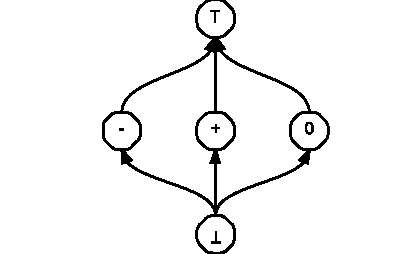
\includegraphics{img/lattice.pdf}
  \caption{Bounded lattice with 5 elements.\label{lattice}}    
\end{figure}

        There are several properties of lattices important for DFA.
        
        If we have a finite bounded lattice $(S, \leq_{s})$ and a function 
        $f:S\rightarrow{S}$ that is monotonous, in order words, 
        $\forall{a,b\in{S}}: a\leq_s{b} \Rightarrow f(a)\leq_s{f(b)}$, 
        then $\forall{x\in{S}}$ $\exists{k\in\mathbb{N}}$, such that 
        $f^k(x)=f^{(k+1)}(x)$. $f^k(x)$ is called a fixpoint.
        
        Intuitively, $f$ has to have a fixpoint because 
        for every argument $y$, it must either return 
        $y$ itself, but then $y$ is a fixpoint, or it 
        returns another element that is strictly 
        greater than $y$, but this cannot go on forever, because eventually 
        $f$ will be given $\top$ for which it does not have 
        any other option but returning $\top$ and we 
        have a fixpoint again.
        
        From this property further follows that if we use a finite 
        lattice's elements as a domain for transfer functions, 
        and the transfer functions are monotonous, then the set of 
        data-flow equations has a solution, which is a safe 
        approximation of the, in a sense, best solution to the 
        data flow problem. Details can be found in \cite{kildall1973unified}.
        
        Product lattice obtained from two or more lattices 
        is also a lattice, which can simplify the design of 
        data flow analyses.

        Power set $\mathcal{P}(S)$, the set of all subsets of $S$, 
        is also a lattice, the lattice order relation 
        being subset relation $\subseteq$.

        \subsubsection*{The Iterative Algorithm}
        
        The algorithm to find the solution to the data-flow equations 
        initially sets $OUT(B_i)$ for every basic block to the initial 
        \emph{data-flow}, which should be the lowest element of the lattice. 
        Then it iteratively takes a basic block $B_j$ such that 
        its input \emph{data-flow} $IN(B_j)$ has changed or is not 
        initialized yet and computes $OUT(B_j)$, which might change 
        the input \emph{data-flow} of the ancestors of $B_j$. 
        The process is repeated until a the system stabilizes. 
        
        The algorithm can take basic blocks in any order, however, 
        the \emph{reverse post order} provides the best time complexity 
        \cite{aho1985compilers}.
        
        \subsubsection*{Bit Vectors as Data-flow Representation}

        The performance of the algorithm also depends on the implementation 
        of \emph{data-flow}, the $\textit{MEET}$ operations and the transfer 
        functions. 
        
        \emph{Data-flow} often represents a subset of a set of possible values 
        and the $\textit{MEET}$ operation is either union or intersection.
        For example, a subset of all possible types of a variable. 
        Furthermore, we want to calculate the information for all 
        variables not only for one. If we know the number of variables $n$ and 
        types $m$ in advance, we can represent the \emph{data-flow} as 
        a bit-vector where groups of $m$ bits represent a data of 
        single variable and within those bits, value of bit with 
        index $i$ indicates whether the type with index $i$ is in the set. 
        Union or intersection can be implemented using fast bitwise operations.


        % -----------------------------------------------------------------------
        \subsection{Abstraction}
        
        The \emph{data-flow} value for program point is typically an abstraction 
        of some property of the set of all possible program states that can be 
        observed during real execution for that program point. 
        
        Abstracting the desired property is often important in order to make 
        the analysis practical or even feasible. Let us consider an analysis 
        that should determine the sign of integral variables at each program point.
        We can have inference rules of the following form.
        
        $$
        \infer{[v_3=v_1+v_2, S_1] \rightarrow S_2, S_2 \vdash v_3 : -7 (sign: \ominus)}
        {S_1 \vdash v_1 : -10 (sign: \ominus) & S_1 \vdash v_2 : 3 (sign: \oplus)}
        $$
        
        However, the implementation would not be very efficient and also the full 
        information about variables values is not always available, but in some cases 
        we can deduce another less precise, but still useful piece of information 
        by other means. For example, variable of type \code{unsigned integer} will 
        always be positive, we can count on that even if we do not know the actual value. 
        What we can do is to abstract the possible integral values with set 
        $\{0, \ominus, \oplus\}$ with the following meanings         
        \begin{itemize}
            \item $\ominus$ represents all negative integers,
            \item $\oplus$ represents all positive integers,
            \item $0$ represents zero,
        \end{itemize}                
        and rewrite the inference rules as follows:
        
        $$
        \infer{[v_3=v_1+v_2, S_1] \rightarrow S_2, S_2 \vdash v_3 : \ominus}
        {S_1 \vdash v_1 : \ominus & S_1 \vdash v_2 : \ominus}
        $$
        
        Nonetheless, there is another problem. What to do when we have $\ominus$ 
        and $\oplus$ in the hypothesis.
        
        $$
        \infer{[v_3=v_1+v_2, S_1] \rightarrow S_2, S_2 \vdash v_3 : ?}
        {S_1 \vdash v_1 : \ominus & S_1 \vdash v_2 : \oplus}
        $$
        
        The solution is to extend the domain so that it is closed under all operations. 
        We add another element to our set:
        \begin{itemize}
            \item $\top$ represents an unknown value (either positive, negative, or zero).
        \end{itemize}
        Then the rule will be:
        
        $$
        \infer{[v_3=v_1+v_2, S_1] \rightarrow S_2, S_2 \vdash v_3 : \top}
        {S_1 \vdash v_1 : \ominus & S_1 \vdash v_2 : \oplus}
        $$        
        
        And for example another rule dealing with $\top$ in hypothesis:
        $$
        \infer{[v_3=v_1+v_2, S_1] \rightarrow S_2, S_2 \vdash v_3 : \top}
        {S_1 \vdash v_1 : \ominus & S_1 \vdash v_2 : \top}
        $$
        
        It is no surprise that we used symbol $\top$, which is also used to denote the 
        greatest element in a lattice. By adding $\bot$, the least element, and inference 
        rules for it, we can get a lattice depicted in \ref{lattice} and use 
        this abstraction as \emph{data-flow} value.
        
        \subsubsection*{Formalization}

        There is a theoretical framework for designing sound and correct 
        abstractions. In a nutshell, an abstraction following this framework 
        has to include: 
        
        \begin{itemize*}
            \item concrete domain $C$, which has to be a lattice ,
            \item abstract domain $A$, which has to be a finite lattice,
            \item concretization function $\gamma{}:A\mapsto{}C$,
            \item abstraction function $\alpha{}:C\mapsto{}A$,
        \end{itemize*}
        
        In our case the concrete domain could be the power set of all 
        possible integral values, which is a lattice, and the abstract 
        domain with elements $\{0, \ominus, \oplus\, \top, \bot\}$ was 
        described above. The $\gamma$ and $\alpha$ functions map values 
        from one domain to another. When we map elements of concrete domain 
        to the abstract domain, we loose precision due to abstraction. 
        Let us provide few examples, instead of a formal definition 
        of $\gamma$ and $\alpha$.
        
        \begin{align*}
            \begin{split}
                \gamma{}(\oplus) &= \left\{1, 2, 3, ...\right\} \\
                \gamma{}(\top) &= \top = \left\{..., -2, 1, 0, 1, 2, ...\right\} \\
            \end{split}
            \begin{split}
                \alpha{}(\left\{3, 4, 5\right\}) &= \oplus \\ 
                \alpha{}(\left\{3, -4\right\}) &= \top \\
            \end{split}
        \end{align*}
        
        The framework for abstract interpretation further defines 
        necessary conditions for the $\gamma$ and $\alpha$ functions 
        and conditions for the \emph{transfer functions} with respect 
        to $\gamma$ and $\alpha$ mapping. Details and other 
        static analysis methods based on abstract interpretation 
        framework can be found in \cite{cousot1977abstract}, 
        \cite{Cousot2000abstract}.

        % ----------------------------------------------------------------------
        \subsection{Intraprocedural Analysis}
        
        So far we have been discussing an analysis of a single function 
        or a method \footnote{We will use term 
        routine to designate a global function, static or instance method}. 
        However, if we want to analyse a whole program or 
        a library, the interaction between the routines 
        must be taken into account.
        
        A straight forward approach is to regard other routines as 
        black boxes and assume the worst with respect to how a 
        routine call can change the program state. Nonetheless, 
        in practical programming language with references, or pointers,  
        pass-by-reference arguments, lambda functions with 
        capture by reference, and other caveats, an innocent 
        routine call can theoretically do almost anything to 
        the program state even from the local point of view 
        of the function we are analysing.
                
        \subsubsection*{Context Sensitive Intraprocedural Analysis}
        
        The most precise solution is to analyse a function, 
        say \code{foo}, for each possible calling context. 
        In other words, re-analyse \code{foo}'s body every 
        time we encounter its invocation when analysing another 
        function, and use the program state before 
        the invocation of \code{foo} as an initial state 
        for the re-analysis of \code{foo}.
        
        Caching of the results of analysis based on 
        the calling context, so that we do not re-analyse it 
        if the context is the same as some context previously 
        encountered, is possible. However, in the most generic 
        form, it is impossible to asses the equality of 
        program states, because the context consists not only 
        of arguments passed to the function, but also the 
        global state including the heap.
        
        Another problem, which makes fully context sensitive 
        approach impractical or even impossible, is polymorphism 
        or dynamic invocation of routines in general, be it 
        lambda functions, virtual methods, reflection, 
        or any other means. It is not known statically what 
        function will be invoked and thus what function to analyse. 
        The call site can be determined by the analysis itself, 
        but in general it cannot be guaranteed.
        
        \subsubsection*{Heap Abstractions}
        
        When a routine takes a pointer or reference to some object 
        on the heap as an argument, it can traverse to other 
        objects on the heap and change their state. Let alone low-level 
        languages that allow direct manipulation with the memory and 
        can therefore change anything in the heap. 
        
        The heap can be important part of the program state for 
        some kinds of analyses. If we want to take the heap state 
        into the consideration during the analysis, we need an 
        abstraction for the heap to make the approach feasible 
        in practice.
        
        Researchers have proposed several approaches to representation 
        of heap data in an abstract way to minimize memory requirements 
        and provide fast algorithms to check two heap abstractions 
        for equality or isomorphism. A sound and useful definition 
        of heaps isomorphism is also a problematic task by itself. 
        The paper \cite{kanvar2014heap} provides a survey on the heap 
        abstraction models.
        
        \subsubsection*{Region Based Analysis}
        
        Another approach is to analyse a routine once in a 
        generic context setting and create a \emph{transfer function} 
        that summarizes the effects of the routine call to the 
        program state \cite{aho1985compilers}. However, in practical setting, 
        we need to decide how to derive the \emph{transfer function} and how to 
        represent it. A constant \emph{transfer function} that always 
        returns the $\top$, in other words, the worst assumption about 
        the program state, is always safe \emph{transfer function} 
        for any routine call, but we have not gained anything over 
        the naive solution from the beginning of this section.
        
        In the case of Control Flow for Phalanger, we used 
        a variant of a region based analysis. Details are 
        discussed in the following \wsection{}.
    
    % ----------------------------------------------------------------------------
    \section{Control Flow for Phalanger Approach}
        
        \subsection{Assumptions}        
        The approach taken in Control Flow for Phalanger is based on an 
        observation that even when developers are given a dynamically typed 
        programming language, it does not mean that they will write 
        dynamically typed programs. Empirical evidence for this 
        observation was presented in \cite{walker1996type}. 
        
        We are therefore assuming that large part of the analysed 
        code corresponds to a statically typed code one-to-one, 
        it only does not include the type information. However, 
        we do not want to ignore the dynamic typing completely.

        Another decision we made, is that only local variables 
        will be a viable target for compiler optimizations use 
        case, since the compiler optimizations have to be safe with 
        respect to all the possible and obscure corner cases, 
        and global variables and heap memory are difficult to 
        analyse precisely. On the other hand, with bug-hunting and 
        integrated development environment supporting style 
        analyses, we can afford more courageous assumptions.
        
        In this \wsection{} we focus on the type analysis, because 
        it is by far the most complex kind of analysis implemented. 
        Other analyses, like constant propagation, follow the same 
        concepts and, furthermore, they rely on the results of the 
        type analysis and points-to analysis, which is 
        also discussed in this \wsection{}.
        
        \subsection{Analysis Results}
        
        The outcomes of the analysis of a single routine are:
        
        \begin{description*}
            \item[Variables table: type information for local variables] -- 
            for every local variable, a set of its possible types at any 
            point during the execution of the routine. Note that it summarizes 
            all types that variable can have at different program points. 
            Knowing that a variable has only one possible type can be useful 
            for compiler.
            
            \item[Type information for expressions] -- every expression in the 
            routine's body will be annotated with the type or set of types 
            the expression can evaluate to.
            
            \item[Warnings] -- some expressions expect only operands of 
            certain type; if the analysis encounters such expression 
            and from the analysis it follows that the operand is not of the 
            expected type, the piece of code in question is reported as a warning.
            The same holds for the type expectations extracted from 
            documentation comments for fields, routines and others.
            
        \end{description*}
        
        Another outcome of analysis across all routines will be \emph{globals table} 
        with type information for global symbols that is global variables, 
        instance and static fields and routines.
        
        \subsection{Local Analysis: Overview}
        
        We can think about expressions in terms of 
        evaluation trees, like in figure \ref{evaltree}. 
        Since expressions should be annotated with their 
        type information, the analysis can use a bottom 
        up approach and annotate the leaves of the 
        evaluation tree first and then recursively from 
        the type information of operands infer type 
        information for compound expressions.
        
        \begin{figure}[h]  
          \centering        
          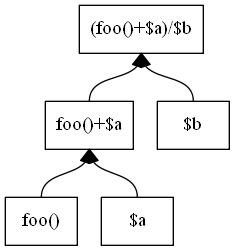
\includegraphics[scale=0.5]{graphs/evaltree.png}
          \caption{Evaluation tree of an expression \code{(foo()+\$a)/\$b}.\label{evaltree}}    
        \end{figure}        
        
        Statements or expressions that can change the program state, 
        like assignment statement, will have their operands 
        annotated with the type information and thus have all 
        the necessary information to reflect the change of 
        the program state accordingly. For instance, 
        the type of the right hand side expression of an assignment 
        statement will determine the new type for the variable 
        on the left hand side.
        
        Some type information can be inferred from the code without 
        any knowledge about variables' types. For example, the result 
        of string concatenation is always a \code{string}, no matter 
        what the types of the arguments are. However, simple local 
        variable use is an expression and we need to know the possible 
        types of the variable to annotate this expression 
        with its type. For this, we need to perform a DFA that will 
        give us the type information for each variable at each program 
        point. Note that the \emph{data-flow} values are used only 
        temporarily to annotate the expressions and build the variables 
        table, but we do not create actual \emph{data-flow} instance 
        for every program point.
        
        The questions that have to be answered, in order to 
        implement the DFA, include:
        
        \begin{itemize*}
            \item what the \emph{data-flow} values will be, 
            \item what data structures will be used to represent them efficiently, 
            \item how to deal with routines calls and their effects to the program state.
        \end{itemize*}
        
        \subsection{Local Analysis: Data-flow Values}
        
        The \emph{data-flow} should capture the type information 
        for variables within the routine. We do want to support 
        dynamic typing, therefore for every variable, we have 
        a subset of all its possible types, not only a single type.        
        The \emph{data-flow} value is a map from variable names to 
        subsets of types. 
        
        For an efficient representation of the \emph{data-flow}, 
        the routine's body is scanned for all local variables names 
        referenced types prior to the analysis. After the scan, the 
        number of variables and types is a known constant and the 
        \emph{data-flow}, being an array of subsets of a set 
        of all the types, can be represented as a bit-vector. 
        The $\operatorname{MEET}$ operation is a union, because if 
        a variable can have type \code{T} from one branch and 
        type \code{K} from another, at the join point we can only 
        assume that it has either type \code{T} or \code{K}.
        
        However, with a real world class based object oriented 
        programming language, the situation is not as simple. 
        We have to deal with subtyping, and we also want to 
        support type information from documentation comments, 
        which nonetheless should be distinguished from the 
        type information inferred from the actual code.
        
        The basic \emph{data-flow} values for a single variable 
        and set of types $\left\{int, false, null\right\}$ are depicted 
        in the figure \ref{typeslattice1}. Aside the whole set of 
        all types references within the routine's body, we have 
        another artificial value called \emph{Any}, which simply 
        designates any possible type, not restricted to the set 
        of known types. In the following paragraphs, we discuss 
        how we added support for classes and documentation 
        comments to this schema. We focus on \emph{data-flow} 
        lattice for a single variable; the lattice for all variables 
        will simply be a product lattice.
        
        \begin{figure}[h]  
          \centering        
          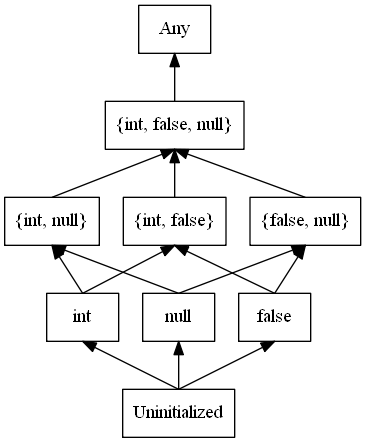
\includegraphics[scale=0.6]{graphs/types-lattice1.png}
          \caption{Basic lattice with types.\label{typeslattice1}}    
        \end{figure}
        
        \subsubsection*{Booleans}        
        In the case of booleans, we distinguish 
        \code{true} and \code{false}, because it is a well 
        known pattern in PHP for routines to use \code{false} 
        return value as an indication of failure. 
        Routines then can have, for example, have type 
        \code{false|object} meaning that this routine returns either 
        object or value \code{false}, never value \code{true}.
        
        \subsubsection*{Null}        
        Another thing to note is that we treat \code{null} as 
        a special type. This again comes from PHPDoc documentation 
        comments, where one can, for instance, state 
        \code{integer|null} as return type of a routine, 
        in which case representing the routines return type 
        as just \code{integer} would not be precise. Moreover, 
        having \code{null} can be used to distinguish between 
        non-nullable and nullable reference types. 
        Control Flow for Phalanger by default assumes that all 
        the reference types can be \code{null}, but it can 
        be configured to assume the opposite, in which case it can, 
        for example, report type error if a routine expects 
        instance of some \code{object} as an argument, 
        but is given \code{null}.
        
        \subsubsection*{Type Hints}        
        We refer to the type information gathered from documentation 
        comments as type hints. For example, routines can have 
        documentation comments that state expected types of the 
        parameters. However, it is perfectly legal to invoke the 
        routine with actual parameters of different types, so we 
        cannot rely on the documentation completely, but we want 
        to utilize it.
        
        For this purpose, we distinguish between type information 
        that was inferred from the code and should always be 
        valid and type information that was extracted from the 
        documentation comments or possibly other unreliable 
        sources, for instance, return type of a non-final method, 
        which cannot be accurately determined because of 
        polymorphism.
        
        The distinction is realized as a single bit flag 
        we call ``type hint''. It is a single flag for the 
        whole set of possible types, so we cannot have a 
        set of two possible types where one is ``type hint'' 
        and the other is not. 
        
        We can think of all the sets with ``type hint'' flag 
        as a parallel lattice to the lattice of sets without 
        ``type hint'' flag. Let us say that $hint(x)$ denotes 
        an element from the parallel lattice corresponding to 
        element $x$ in the original one. If we are comparing 
        two elements $a$ and $b'$, where $b'=hint(b)$ is from the 
        ``type hint'' lattice, we say that their upper bound or 
        supremum is equal to $hint(a\wedge{}b)$, formally 
        $a\wedge{}b'=hint(a\wedge{}b)$. A lattice that is formed 
        from putting together the original types lattice and the 
        ``type hint'' lattice for types $\left\{int, string\right\}$ 
        is depicted in figure \ref{hintslattice}.
        
        \begin{figure}[h]  
          \centering        
          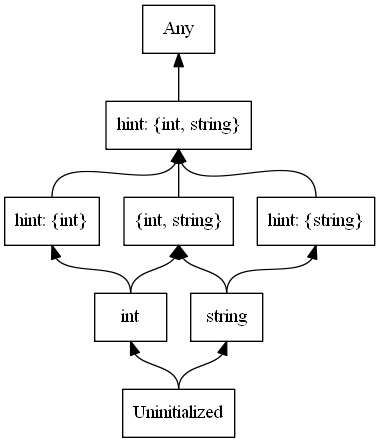
\includegraphics[scale=0.6]{graphs/hints-lattice.png}
          \caption{Types lattice with ``type hint'' flag.\label{hintslattice}}    
        \end{figure}
        
        
        \subsubsection*{Classes}
        
        We refer to built-in types as basic types, those are 
        \begin{multicols}{2}
        \begin{itemize*}
            \item int
            \item double
            \item string
            \item resource
            \item false and true (instead of boolean)
            \item null
            \item array
            \item callable -- for example: lambda
        \end{itemize*}
        \end{multicols}
        
        If we say that variable \code{\$a} is of type \code{T}, 
        where \code{T} is a non-final class, even in statically 
        typed language, this could mean that \code{\$a} can 
        be in fact instance of many different classes, 
        namely \code{T} and all its subclasses.
        
        Because we are in a dynamic environment, we cannot, 
        in general, know all subclasses of \code{T} in advance. 
        Nonetheless, it can be useful to distinguish between 
        ``\code{\$a} is of type \code{T} only'' and 
        ``\code{\$a} is of type \code{T} or any of its subtypes''.
        
        To make this distinction, we add another flag ``subclasses'', 
        which works similarly to ``any type'' flag: it holds or does 
        not hold for the whole set of class types. Also the upper bound 
        of two elements, where one of the has the flag ``subclasses'', 
        will has the ``subclasses'' flag.
        
        Moreover, we add one artificial value, which is \code{object}, 
        and it denotes arbitrary class instance, but it is not the 
        same as \emph{Any}, because it excludes the other primitive 
        types. A lattice for just class types $\left\{T,K\right\}$ 
        is in figure \ref{objectslattice}.
        
        \begin{figure}[h]  
          \centering        
          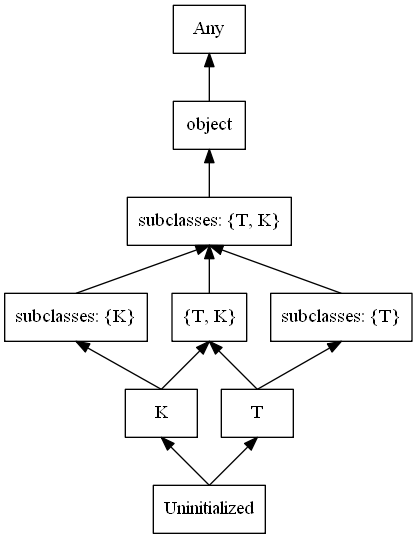
\includegraphics[scale=0.5]{graphs/objects.png}
          \caption{Types lattice with classes.\label{objectslattice}}    
        \end{figure}        
        
        The upper bound of any set of class types and a set of 
        basic types is a union of those. However, the upper 
        bound of a set with some class types in it and a set with 
        \code{object} in it is a union of the basic types and 
        \code{object}, so the class types are ``overridden'' by 
        the \code{object}. This is illustrated in figure \ref{objectsandbasics}.
        
        \begin{figure}[h]  
          \centering        
          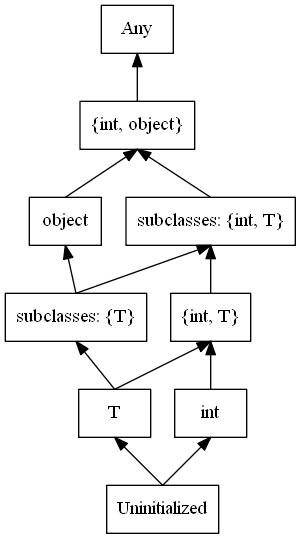
\includegraphics[scale=0.5]{graphs/objects-prim.png}
          \caption{Types lattice: class and a basic type.\label{objectsandbasics}}    
        \end{figure}
        
        This lattice with class types can be amended with the ``type hint'' 
        flag the same way we did before we introduced classes.
        
        \subsection{Intraprocedural Analysis}
        
        The approach we described so far considers only local variables, 
        but we want to analyse object and class fields' types, and global 
        variables. We also have to take into account possible changes to 
        local variables made from other routines through references.
        
        The assumption here is that the results of analysis for fields 
        and global variables do not have to be precise and that although 
        PHP is a dynamic language that permits dynamic fields and dynamic 
        methods, mostly the developers do not abuse those features and 
        we can assume that instances of the same class have the same 
        fields of the same type and the same methods across the whole 
        program. Furthermore, routines return type and expected 
        arguments types will mostly be constant and independent 
        from the program state or each other.
        
        \subsubsection*{Routines Return Values}
        When the analysis encounters a routine invocation, it needs 
        to know the routine's return type and possible other pieces 
        of information we discuss later.
        
        If the source code of the routine in question is available, 
        in other words, it is part of the analysed source, we 
        recursively trigger its analysis in order to infer its 
        return type. When the analysis finished, we save the 
        results to the \emph{globas table} so that we do not 
        need to analyse the routine next time and resume the 
        analysis of the original routine.
        
        This approach, however, does not work for recursive 
        and mutually recursive routines. The solution we use 
        is that if a cycle in routines invocations is detected, 
        we do not analyse the last routine in the cycle, but 
        instead we assume the worst about its return type -- 
        we assume it can return any type.
        
        
        \subsubsection*{Heap}        
        Let us first provide an example, where heap abstraction and 
        context sensitive intraprocedural analysis would be useful:
        
%pygmentize_begin php
% function foo() {
%   $a = new X();
%   boo($a);
%   return $a->bar;
% }
%
% function boo(X $a) {
%   $a->bar = 3;
% }
%pygmentize_end
        
        Here the function \code{boo} changes type of the nested field 
        \code{bar}. If we do not reflect this in the program 
        state after the invocation of \code{boo(\$a)} in 
        function \code{foo}, we cannot determine the type of 
        the return expression \code{\$a->bar}.
        
        However, we decided to approach this problem differently. 
        We do not analyse individual object instances, 
        instead we summarize the type information inferred 
        for individual instances of the same class and provide 
        those results within the \emph{globals table}.
        
        Illustrated on the same example, when analysing function 
        \code{foo}, the analysis would encounter the invocation 
        of \code{boo}. Since \code{boo} has not been analysed yet, 
        this triggers analysis of \code{boo}. While analysing 
        \code{boo} the \emph{globals table} learns that 
        field \code{bar} can be of type \code{integer}. When analysis 
        of \code{boo} finishes and analysis of \code{foo} resumes, 
        on the line with \code{return \$a->bar} we know from the 
        \emph{data-flow} that \code{\$a} is of type \code{X} and 
        from the \emph{globals table} we get that field \code{bar} 
        of class \code{X} can be of type \code{integer}.
        
        With this approach we do not have to model heap, 
        which can be more effective, but on the other hand, 
        there are cases different to this example, where our 
        approach fails to devise any useful information 
        and heap model, could give us 
        better results. For instance, if function \code{boo} 
        did not provide type information for its parameter 
        in its signature, because we analyse each routine 
        in a generic context.
                
        Moreover, we ignore the effects of indirect assignments 
        and references to the \emph{globals table}, which means 
        that the \emph{globals table} is not safe approximation. 
        However, as we stated at the beginning of this \wsection{}, 
        the analysis of instance fields is meant for bug hunting 
        purposes and we can afford some imprecision. In addition, 
        the type information inferred by means of \emph{globals table} 
        is marked with the ``type hint'' flag.
        
        The global variables and static class field are analysed 
        in the way as instance fields.
        
        \subsubsection*{Type Documentation}
        There are two different cases where we need to consider type 
        information for fields or global variables: when a field or global 
        variable is read, and when a field or global variable is assigned to.
        
        Field and global variables can have PHPDoc type documentation.
        In the case of assignment, we want to check that the value assigned 
        to the variable has a type compatible with the documentation, 
        otherwise it is possibly a bug or documentation error.
        
        When it comes to type annotation of an expression that uses 
        a global variable or a field, if the type documentation is available, 
        we use it over the information from \emph{globals table}, 
        but still mark the type information with ``type hint'' flag.
        
        \subsubsection*{References Analysis}
        References in PHP are used, but occasionally, therefore we do 
        not want to ignore them, but we do not require a 
        precise results when references are used in 
        the analysed routine.
        
        Another piece of information the analysis needs to know 
        about a routine that is being invoked from within the 
        analysed routine is which arguments are passed by reference 
        to it, so that their value can be changed inside the 
        invoked function. This is fortunately a part of the 
        routine's signature, and can be easily determined. 
        We simply throw away any assumptions we had about the type 
        of a variable which is being passed by reference to 
        another routine.
        
        The situation is more complicated with references within a 
        single routine. When a statement or expression can change 
        the type of a variable, it can change type of any variable 
        that this variable points to, if it is a reference.
        
        We use a simple approach: prior to the analysis, the routine 
        body is scanned for any assignments by reference (\code{\$a=\&\$b}) 
        and two sets are created: variables that can be a reference and 
        variables that can be pointed to by a reference. This is very 
        conservative approximation, but we expect sparse usage of 
        references.
        
        When the analysis finds out that a type of a variable can 
        be changed to \code{T}, it checks if the variable can be 
        a reference and if so the types of all the variables that 
        can be pointed to by any reference are updated. Those variables 
        \textbf{may} only be pointed to, but do not \textbf{have to} 
        be pointed to, so we take their current type information 
        and merge with type \code{T}, creating over approximation.
        
        Moreover, any routine's invocation can change any local 
        variable from the can be pointed to set, because 
        references can ``leak'' on the heap, for where 
        the other routine can read them. That is why, after any routine 
        invocation, we throw away any assumptions about variables 
        in the can be pointed to set.
        
        The same holds for local variables that are captured by 
        reference by some lambda function. The lambda function can 
        again ``leak'' on the heap, from where the other routine 
        can invoke it.
        
        %TODO: \subsubsection*{Arrays}
        
        